\section{Mission Overview}
The root requirement of a satellite-based ADS-B system was the provision of ADS-B coverage over regions where terrestrial systems did not currently provide coverage (in particular, oceans and poles). Within this requirement were a number of variable mission parameters that effected the design and economic cost of resulting satellite systems. Varying the parameters and analysing the performance of resulting designs was used for a mission trade-off analysis, presented in Section \ref{sec:decision_matrix}.

\subsection{System Users}
A spaced based ADS-B system would have two key user groups
\begin{itemize}
	\item Air Navigation Service Providers
	\item Airlines and air transportation service providers
\end{itemize}
Although Australia, America and Europe were able to implement terrestrial ADS-B stations, rolling out terrestrial stations to cover all interest areas was not necessarily cost effective. This was particularly true in regions such as South East Asia. In such areas, the technology and economic base did not exist to make terrestrial deployment viable \cite{Blomenhofer2012}. In these situations a satellite-based system could more effectively augment existing ADS-B coverage for use by ANSPs.

Another key user would be airlines and other air transportation services. Greater position and telemetry coverage of aircraft over oceanic and polar regions would facilitate more optimal flight path co-ordination. ADS-B assisted flight routing would allow for narrower longitudinal and latitudinal track separation, allowing for more flights to travel on desired fuel-saving paths. A flight simulation analysis presented by Iridium LLC suggests that increased density of planes in jet streams can result in fuel savings of up to 450 litres per oceanic flight \cite{Dawson2013}. 


\subsection{System Update Rate}
The update rate of a space-based ADS-B system defined timeliness with which aircraft data can be updated and disseminated terrestrially. Having a high-effective update rate was crucial in range of Airports with ATC towers having to co-ordinate a large density of aircraft traffic. With ADS-B, terrestrial ATC towers typically achieved an update rate of less than 1 second depending on airport capacity \cite{Orlando2001}. For the purposes of live tracking and safety control, an update rate in the order of 1 second to 30 seconds would be required. An update rate in the order of 5 to 10 minutes would enable satisfactory tracking by airlines and air transport services at less cost. A lowest cost system with an update rate of 1-2 hours could be useful for occasional tracking of aircraft making oceanic flights. This, however, would be inadequate for safety applications or any short-range terrestrial flights. 

\subsection{Revisit Time}
Due to the random access nature of Mode S Extended Squitter, the number of aircraft surveyed by an ADS-B receiver was limited. Scanning for a shorter period, or scanning an area with more aircraft would result in more ADS-B collisions and a drastically reduced detect rate. `Missing' aircraft in this manner would be unacceptable from a safety perspective. Suggested solutions for high density areas included more sophisticated antenna design with spot beams \cite{Blomenhofer2012}, or variable-periodicity of ADS-B signals \cite{Orlando2001}. 

For ADS-B reception via satellite, a populated area could be either scanned for a longer period, or `re-scanned' over multiple revisits. This would mediate the need for a larger or more sophisticated and costly antenna array. A longer scanning period could be achieved slowing the ground-track of the space segment over key areas. This would particularly be a problem on CubeSats where technology capability was limited. The revisit time would therefore be defined by limitations of the antennae array and on-board processing technology for ADS-B signal reception. More detail on current small-satellite ADS-B receiver research is discussed in Section \ref{sec:litreview}.
 
\subsection{Geographical Coverage}
Full global coverage would be achieved by a series of polar or near polar orbits, such as the Iridium Satellite constellation \cite{iridium_ICAO_man,iridium:an_overview1998}. Achieving full coverage would be the most costly solution, requiring the largest number of satellites and ground stations. At the very least, the ADS-B system should at least cover the North Atlantic, North Pacific and Indian Oceans and South East Asia in order to meet the root system requirement. These areas had the highest amount of air traffic not covered by terrestrial ADS-B systems as shown in Figure \ref{fig:flightpaths}. Monitoring these regions with specific orbits can reduce the number of spacecraft required in order to provide the coverage gap required by the system. Coverage of the poles would provide extra benefit, opening up polar flight paths.
\begin{figure}[htbpp]
	\centering
	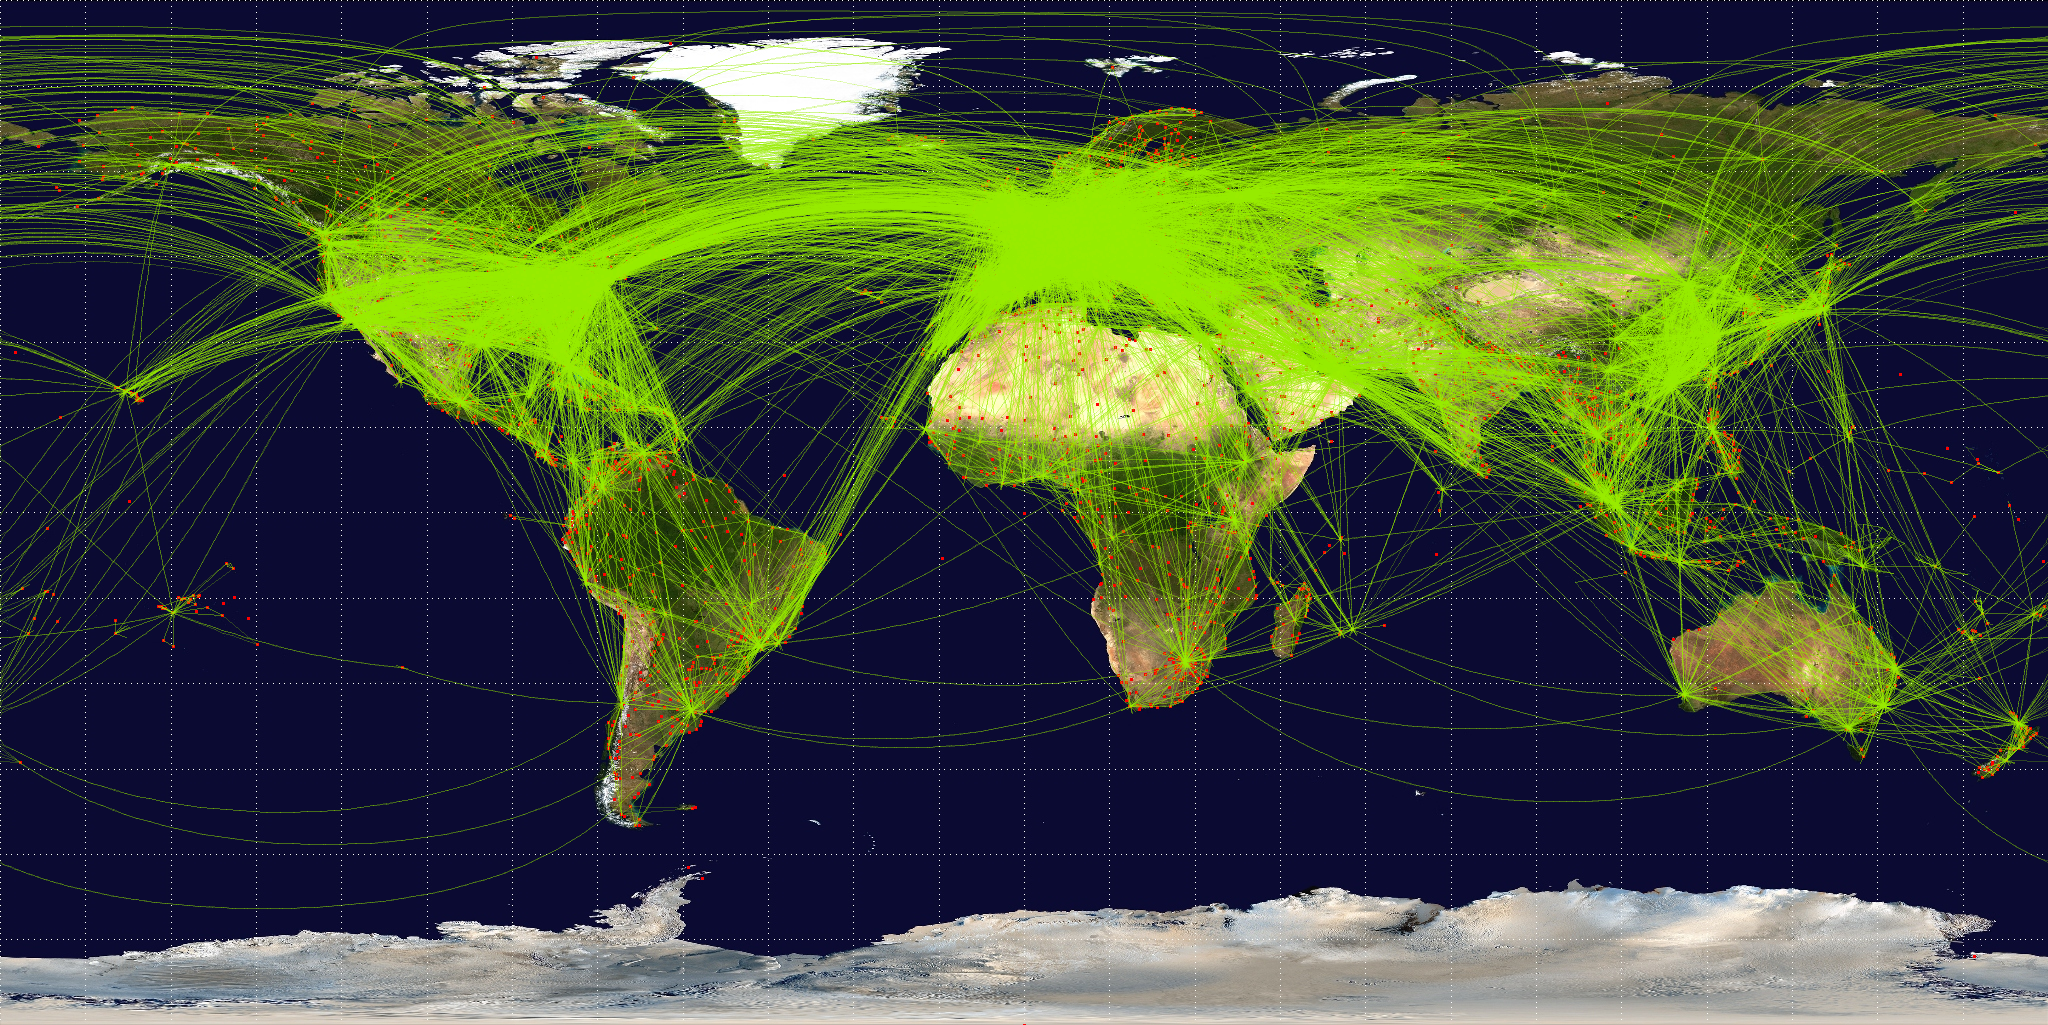
\includegraphics[scale = 0.18]{Pictures/flightpaths.png}
	
	\caption[Popular flight routes]{Popular flight routes, from \cite{Open}}
	\label{fig:flightpaths}
\end{figure} 


